\chapter{Vectors}
\section{Introduction}
There are three common ways to describe a vector:
\begin{itemize}
  \item \textbf{"The Physicist's definition"}: An object that has a magnitude and a direction (a geometric definition).
  \item \textbf{"The Computer scientists' definition"}: An array of numbers (an arithmetic definition).
  \item \textbf{"The Mathematician's definition"}: An element of a vector space (an abstract definition).
\end{itemize}
In this course we will introduce the physicist's (geometric) approach first, then the computer scientists' (arithmetic) approach, linking the two approaches together.\\ The mathematician's (abstract) approach will remain mostly untouched until the last chapter where we generalize the definition of a vector.

\section{Geometric Approach}
\subsection{Basics}
A \emph{vector}\index{Vector} is an object that has a \emph{magnitude}\index{Magnitude of a vector} (also a \emph{norm}\index{Norm of a vector}, or a \emph{length}\index{Length of a vector}), and a \emph{direction}\index{Direction of a vector} (also an \emph{argument}\index{Argument of a vector}). A vector starts at a point (called its \emph{origin}\index{Origin of a vector space}), and ends at a point. We draw vectors as arrows starting at the start point with their head at the end point.
\begin{example}
  Some 2-dimensional vectors having different starting and ending points:
  \begin{figure}[H]
  \centering
  \begin{tikzpicture}
  \draw[vector, col1] (0,0) -- (2,3);
  \draw[vector, col2] (-1,0) -- (-2,2);
  \draw[vector, col3] (0,-1) -- (-3,-1);
  \draw[vector, col4] (2,0) -- (1,-3);
  \draw[vector, col5] (-4,2) -- (-4,-2);
  \draw[vector, black] (-7,1) -- (-6,0);
  \end{tikzpicture}
  \end{figure}
\end{example}
In physics (and this course), vectors are usually notated by undercase Latin letters with a small right-facing arrow drawn above them, i.e.:
\begin{equation*}
  \vec{u},\quad\vec{v},\quad\vec{x},\quad\vec{a},\quad\dots
\end{equation*}
However, mathematicians tend to write vectors as undercase Latin letters that are either bold faced, with or without an underline, i.e.:
\begin{align*}
  \bm{u},\quad\bm{v},\quad\bm{x},\quad\bm{a},\quad\dots\\
  \underline{\bm{u}},\quad\underline{\bm{v}},\quad\underline{\bm{x}},\quad\underline{\bm{a}},\quad\dots\\
\end{align*}
We consider all vectors to originate in the same point (which we call the \emph{origin}\index{Origin of a vector space}).
\begin{example}
  The 2-dimensional vectors from before, placed such that they originate from the same point:
  \begin{figure}[H] 
  \centering
  \begin{tikzpicture}
  \draw[vector, col1] (0,0) -- (2,3);
  \draw[vector, col2] (0,0) -- (-1,2);
  \draw[vector, col3] (0,0) -- (-3,0);
  \draw[vector, col4] (0,0) -- (-1,-3);
  \draw[vector, col5] (0,0) -- (0,-4);
  \draw[vector, black] (0,0) -- (1,-1);
  \filldraw[black] (0,0) circle (0.05);
  \end{tikzpicture}
  \end{figure}
\end{example}

\subsection{Scaling a Vector, Adding Vectors}
\newcommand{\vecu}{
  \color{col1}{\vec{u}}\color{black}
}
\newcommand{\vecv}{
  \color{col2}{\vec{v}}\color{black}
}
\newcommand{\vecw}{
  \color{col3}{\vec{w}}\color{black}
}
Scaling a vector changes its magnitude without changing its direction. This is done by multiplying the vector by a real number, which in this context we call a \emph{scalar}\index{Scalar}.
\begin{example}
  Scaling a vector $\vec{v}$ by $2,3,-1$ and $-2$:
  \begin{figure}[H]
  \centering
  \begin{tikzpicture}
  \Large
  \draw [vector, col1] (0,0) -- ++(1.5,1) node [midway, above] {$\vec{v}$};
  \draw [vector, col2] (2,0) -- ++(3,2) node [midway, above] {$2\vec{v}$};
  \draw [vector, col4] (4,0) -- ++(4.5,3) node [midway, above, xshift=-1mm] {$3\vec{v}$};
  \draw [vector, <-, thick, col6] (6,0) -- ++(1.5,1) node [midway, above, xshift=-2mm] {$-1\vec{v}$};
  \draw [vector, <-, thick, black] (8,0) -- ++(3,2) node [midway, above, xshift=-2mm] {$-2\vec{v}$};
  \end{tikzpicture}
  \end{figure}
\end{example}
\begin{warning}
  Notice that scaling a vector by a negative number reverses its direction.
\end{warning}
Adding two vectors is done by placing the origin of one vector at the head of the other vector. The addition result is a vector starting at the first vector's origin and ending at the second vector's head.

\begin{example}
  Adding two vectors $\vecu$ and $\vecv$ according to the above scheme:
  \begin{enumerate}
  \item The two vectors $\vecu$ and $\vecv$ originating from the same point
  \item Moving $\vecv$ so that its origin is placed at the head of $\vecv$.
  \item Drawing a vector $\rcolor{col4}{\vec{w}}=\vecu+\vecv$ from the origin of $\vecu$ to the head of $\vecv$.
  \item Moving $\vecv$ back to the origin.
  \end{enumerate}
  \begin{figure}[H]
  \renewcommand\thesubfigure{\arabic{subfigure}}
  \begin{subfigure}[t]{0.5\textwidth}
  \centering
  \begin{tikzpicture}
  \Large
  \coordinate (o) at (0,0);
  \coordinate (u) at (-2,1);
  \coordinate (v) at (3,2);
  \coordinate (w) at ($(u)+(v)$);
  \draw[vector, col1] (o) -- ++(u) node[left] {$\vec{u}$};
  \draw[vector, col2] (o) -- ++(v) node[right] {$\vec{v}$};
  \filldraw[black] (o) circle (0.05);
  \end{tikzpicture}
  \caption{}
  \end{subfigure}
  \begin{subfigure}[t]{0.5\textwidth}
  \centering
  \begin{tikzpicture}
  \Large
  \draw[vector, col1] (o) -- ++(u) node[left] {$\vec{u}$};
  \draw[vector, col2] (u) -- ++(v) node[right] {$\vec{v}$};
  \filldraw[black] (o) circle (0.05);
  \end{tikzpicture}
  \caption{}
  \end{subfigure}
  \par\bigskip
  \begin{subfigure}[t]{0.5\textwidth}
  \centering
  \begin{tikzpicture}
  \Large
  \draw[vector, col1] (o) -- ++(u) node[left] {$\vec{u}$};
  \draw[vector, col2] (u) -- ++(v) node[right] {$\vec{v}$};
  \draw[vector, col4] (o) -- node [midway, right] {$\vec{w}=\rcolor{col1}{\vec{u}}+\rcolor{col2}{\vec{v}}$} ++(w) ;
  \filldraw[black] (o) circle (0.05);
  \end{tikzpicture}
  \caption{}
  \end{subfigure}
  \begin{subfigure}[t]{0.5\textwidth}
  \centering
  \begin{tikzpicture}
  \Large
  \draw[vector, col1] (o) -- ++(u) node[left] {$\vec{u}$};
  \draw[vector, col2] (o) -- ++(v) node[right] {$\vec{v}$};
  \draw[vector, col4] (o) -- ++(w) node[right] {$\vec{w}$};
  \filldraw[black] (o) circle (0.05);
  \end{tikzpicture}
  \caption{}
  \end{subfigure}
  \end{figure}
\end{example}

The order of addition does not change the result:
\begin{equation*}
  \vec{u} + \vec{v} = \vec{v} + \vec{u}.
\end{equation*}

This property is known as \emph{commutativity}\index{Commutativity}.

\begin{example}
  Adding the vectors $\vecu,\vecv$ in two ways: first by moving $\vecv$ so that its origin is at the head of $\vecu$, and then by moving $\vecv$ such that its origin is at the head of $\vecu$. Both additions result in the same vector $\vec{w}$. The drawn addition method is known as the \emph{parallelogram}\index{Parallelogram} method.
  \begin{figure}[H]
  \renewcommand*\thesubfigure{\arabic{subfigure}}
  \begin{subfigure}[b]{0.5\textwidth}
  \centering
  \begin{tikzpicture}
  \draw[vector, col1] (o) -- ++(u) node [midway, above] {$\vecu$};
  \draw[vector, col2] (o) -- ++(v) node [midway, above] {$\vecv$};
  \filldraw[black] (o) circle (0.05);
  \end{tikzpicture}
  \caption{}
  \end{subfigure}
  \begin{subfigure}[b]{0.5\textwidth}
  \centering
  \begin{tikzpicture}
  \draw[vector, col1] (o) -- ++(u) node [midway, above] {$\vecu$};
  \draw[vector, col2] (o) -- ++(v) node [midway, above] {$\vecv$};
  \draw[vector, col1] (v) -- ++(u) node [midway, above] {$\vecu$};
  \draw[vector, col2] (u) -- ++(v) node [midway, above] {$\vecv$};
  \draw[vector, col4, dashed] (o) -- ++(w) node [midway, above, xshift=-0.15cm] {$\vec{w}$};
  \filldraw[black] (o) circle (0.05);
  \end{tikzpicture}
  \caption{}
  \end{subfigure}
  \end{figure}
\end{example}

One special vector is the \emph{zero vector}\index{Zero vector} $\vec{0}$, which has a norm of $0$ and no direction. The zero vector is neutral to addition:
\begin{equation*}
  \vec{v} + \vec{0} = \vec{0} + \vec{v} = \vec{v}.
\end{equation*}

\newpage
\section{Algebraic Approach}
\subsection{Basics}
We can place all vectors on an axis system, such that their origins are placed at $x=0, y=0$:
\begin{figure}[H]
  \centering
  \begin{tikzpicture}[every path/.style={->, >=stealth, very thick},
  scale=2.0]
  % Labels size
  \Large

  % Coordinate
  \coordinate (u) at (2,1.5);
  \coordinate (v) at (-2,1);
  \coordinate (w) at (-1,2.5);
  \coordinate (a) at (1,-2);
  \coordinate (b) at (-0.5,-2.5);

  % Axes
  \draw[<->] (-3,0) to (3,0) node [right] {$x$}; 
  \draw[<->] (0,-3) to (0,3) node [above] {$y$};

  % Vectors
  \draw[col1] (o) -- ++(u) node [midway, left, yshift=2mm] {$\vec{u}$};
  \draw[col2] (o) -- ++(v) node [midway, left, yshift=-2mm] {$\vec{v}$};
  \draw[col3] (o) -- ++(w) node [midway, left] {$\vec{w}$};
  \draw[col4] (o) -- ++(a) node [midway, left, yshift=-2mm] {$\vec{a}$};
  \draw[col5] (o) -- ++(b) node [midway, left] {$\vec{b}$};
  \end{tikzpicture}
\end{figure}

For each vector, we can drop a line perpendicular from its head to the $x$-axis. We label the intercept point with the $x$-axis as $u_{x}$:
\begin{figure}[H]
  \centering
  \begin{tikzpicture}[every path/.style={->, >=stealth, very thick},
  scale=2.0]
  % Labels size
  \Large

  % Axes
  \draw[<->] (-1,0) to (3,0) node [right] {$x$}; 
  \draw[<->] (0,-1) to (0,3) node [above] {$y$};

  % Vector
  \draw[-, densely dotted, black!25] (o)++(u) -- (u|-o);
  \draw[col1] (o) -- ++(u) node [midway, left, yshift=5mm] {$\vecu$};
  \draw[-, thick] (u|-o)++(0,-0.1) --++(0,0.2) node [below, yshift=-5mm] {$u_{x}$};
  \end{tikzpicture}
\end{figure}
Similarly, we drop a line from the head of the vector perpendicular to the $y$-axis, and label the intercept point as $u_{y}$:
\begin{figure}[H]
  \centering
  \begin{tikzpicture}[every path/.style={->, >=stealth, very thick},
  scale=2.0]
  % Labels size
  \Large

  % Axes
  \draw[<->] (-1,0) to (3,0) node [right] {$x$}; 
  \draw[<->] (0,-1) to (0,3) node [above] {$y$};

  % Vector
  \draw[-, densely dotted, black!25] (o)++(u) -- (u-|o);
  \draw[col1] (o) -- ++(u) node [midway, left, yshift=5mm] {$\vecu$};
  \draw[-, thick] (u-|o)++(-0.1,0) --++(0.2,0) node [left, xshift=-5mm] {$u_{y}$};
  \end{tikzpicture}
\end{figure}

We write the vector as a \emph{column vector}\index{Column vector} as follows:
\begin{equation*}
  \vec{u}=\colvec{2}{u_{x}}{u_{y}}
\end{equation*}
we refer to the entries of the vector as its \emph{components}\index{Components of a vector} or \emph{coordinates}\index{Coordinates of a vector}. The vector $\vec{u}$ is an element in the set $\Rs{2}$.
\begin{warning}
  We can also write the vector as a \emph{row vector}\index{Row vector}:
  \begin{equation*}
  \vec{u} = \left( u_{x}, u_{y} \right)
  \end{equation*}
  but in some applications (e.g. Tensor analysis) this has a different meaning, and so in this course we will stick with column vectors.
\end{warning}

In 3-dimensions (also called $\Rs{3}$) the principal is the same:
\begin{figure}[H]
  \centering
  \begin{tikzpicture}[every path/.style={->, >=stealth, very thick},
  scale=1.5]
  \coordinate (O) at (0,0,0);

  \Large

  \pgfmathsetmacro{\vx}{3};
  \pgfmathsetmacro{\vy}{2};
  \pgfmathsetmacro{\vz}{2};
  \coordinate (v) at (\vx,\vy,\vz);
  \coordinate (vxz) at (\vx, 0, \vz);

  \pgfmathsetmacro{\alen}{4};
  \draw[->, col1, thick] (o) to (\alen,0,0) node [right] {$x$};
  \draw[->, col2, thick] (o) to (0,\alen,0) node [above] {$y$};
  \draw[->, col3, thick] (o) to (0,0,\alen) node [below left] {$z$};

  \draw[->, >=stealth] (O) to (v) node [above right] {$\vec{v}$};
  \draw[-, dashed, col1] (vxz) -- (\vx,0,0) node [above] {$v_{x}$};
  \draw[-, dashed, col2] (v) -- (vxz);
  \draw[-, dashed, col2] (v) -- (0,\vy,0) node [left] {$v_{y}$};
  \draw[-, dashed, black!20] (vxz) -- (O);
  \draw[-, dashed, col3] (vxz) -- (0,0,\vz) node [left] {$v_{z}$};
  \end{tikzpicture}
\end{figure}

As a column vector, the zero vector has all-zero components. In $\Rs{2}$ this means:
\begin{equation*}
  \vec{0} = \colvec{2}{0}{0}
\end{equation*}
and in $\Rs{3}$:
\begin{equation*}
  \vec{0} = \colvec{3}{0}{0}{0}
\end{equation*}

\begin{example}
  For each of the follows vectors in $\Rs{2}$, we will find its components:
  \begin{figure}[H]
  \centering
  \begin{tikzpicture}[every path/.style={->, >=stealth, very thick},
  scale=1.5]
  \Large

  \coordinate (u) at (2,1);
  \coordinate (v) at (-2,1);
  \coordinate (w) at (-3,3);
  \coordinate (a) at (1,-3);
  \coordinate (b) at (-1,-2);

  \drawaxes{-3}{-3}{3}{3}

  \draw[col1] (o) -- ++(u) node [midway, left, yshift=2mm] {$\vec{u}$};
  \draw[col2] (o) -- ++(v) node [midway, left, yshift=-2mm] {$\vec{v}$};
  \draw[col3] (o) -- ++(w) node [midway, above right] {$\vecw$};
  \draw[col4] (o) -- ++(a) node [midway, left] {$\vec{a}$};
  \draw[col5] (o) -- ++(b) node [midway, left] {$\vec{b}$};
  \end{tikzpicture}
\end{figure}
\begin{equation*}
  \color{col1}\vec{u} = \colvec{2}{2}{1}\color{black}\quad
  \color{col2}\vec{v} = \colvec{2}{-2}{1}\color{black}\quad
  \color{col3}\vec{w} = \colvec{2}{-3}{3}\color{black}\quad
  \color{col4}\vec{a} = \colvec{2}{1}{-3}\color{black}\quad
  \color{col5}\vec{b} = \colvec{2}{-1}{-2}\color{black}
\end{equation*}
\end{example}

\subsection{Scaling a Vector, Adding Vectors}
Column vectors are scaled by multiplying each of their components by the same scalar.
\begin{example}
  \begin{align*}
  \vec{u} &= \colvec{2}{1}{-3}\quad\Rightarrow\quad2\vec{u}=\colvec{2}{2}{-6},\quad -3\vec{u}=\colvec{2}{-3}{9}\\
  \vec{v} &= \colvec{3}{-2}{0.5}{1}\quad\Rightarrow\quad4\vec{v}=\colvec{3}{-8}{2}{4},\quad -7\vec{u}=\colvec{3}{14}{-3.5}{-7}
  \end{align*}
\end{example}

Two column vectors are added by adding their components \emph{element-wise}\index{Element-wise}.
\begin{example}
  \begin{align*}
  &\vec{u} = \colvec{2}{1}{2},\quad\vec{v} = \colvec{2}{-1}{4},\quad\vec{w}=\colvec{2}{0}{1}\\
  &\vec{a} = \colvec{3}{1}{2}{-3},\quad\vec{b} = \colvec{3}{-1}{4}{0}\\
  &\quad\Downarrow\\
  &\vec{u}+\vec{v} = \colvec{2}{0}{6}\\
  &\vec{u}+\vec{w} = \colvec{2}{1}{3}\\
  &\vec{v}+\vec{w} = \colvec{2}{-1}{5}\\
  &\vec{a}+\vec{b} = \colvec{3}{0}{6}{-3}\\
  \end{align*}
\end{example}
\begin{warning}
  Subtracting a vector from another vector is like adding the first vector to the inverse of the second vector, i.e.
  \begin{equation*}
  \vec{u}-\vec{v} = \vec{u} + (-\vec{v}),
  \end{equation*}
  where $-\vec{v}$ is simply $-1\cdot\vec{v}$.
\end{warning}

Of course, everything written so far is true for vectors of any natural number of components ($n=1,2,3,\dots$). The number of components in a vector is called its \emph{dimension}\index{Dimension of a vector}.
\begin{example}
  Addition of vectors in $\Rs{4}$:
  \begin{equation*}
  \colvec{4}{1}{-2}{0}{7} + \colvec{4}{0}{5}{-2}{2} = \colvec{4}{1}{3}{-2}{9}
  \end{equation*}
  Addition of vectors in $\Rs{5}$:
  \begin{equation*}
  \colvec{5}{1}{-1}{2}{0}{-1} + \colvec{5}{-2}{3}{0}{-1}{1} = \colvec{5}{-1}{2}{2}{-1}{0}
  \end{equation*}
  General Addition of two vectors in $\Rs{n}$:
  \begin{equation*}
  \colvec{4}{x_{1}}{x_{2}}{\vdots}{x_{n}} + \colvec{4}{y_{1}}{y_{2}}{\vdots}{y_{n}} = \colvec{4}{x_{1}+y_{1}}{x_{2}+y_{2}}{\vdots}{x_{n}+y_{n}}
  \end{equation*}
\end{example}
\begin{warning}
  Addition of vectors of different dimensions is \textbf{undefined}!
\end{warning}

\newpage
\section{Norm (Length) and Argument (Angle) of a Vector}
The \emph{norm}\index{Norm of a vector} (or \emph{length}\index{Length of a vector}) of a 2-dimensional vector $\vec{u}$, denoted as $\vnorm{u}$, can be calculated via Pytharogas' theorem:
\begin{figure}[H]
  \centering
  \begin{tikzpicture}[every path/.style={very thick},
  scale=2.0]
  \Large
  \filldraw[thick, fill=col5!20, draw=col5] ($(o)+(u|-o)$) rectangle ++(-0.2,0.2);
  \draw[<->, >=stealth] (-1,0) to (2,0) node [right] {$x$}; 
  \draw[<->, >=stealth] (0,-1) to (0,2) node [above] {$y$};
  \draw[->, >=stealth, col1] (o) -- ++(u) node [midway, above left] {$\vecu$};
  \draw[gray, densely dotted] (u) to ($(o)+(u|-o)$);
  \draw [col4, decorate, decoration={brace, amplitude=3pt, raise=3pt, mirror}]
  (o) -- ($(o)+(u|-o)$) node[midway, yshift=-20pt]{$u_{x}$};
  \draw [col2, decorate, decoration={brace, amplitude=3pt, raise=3pt, mirror}]
  ($(o)+(u|-o)$) -- (u) node[midway, xshift=20pt]{$u_{y}$};
  \end{tikzpicture}
\end{figure}

This results in the norm being:
\begin{equation*}
  \vnorm{u} = \sqrt{u_{x}^{2} + u_{y}^{2}}.
\end{equation*}

\begin{example}
  The norm of $\vec{u}=\colvec{2}{3}{-4}$ is
  \begin{align*}
  \vnorm{u} &= \sqrt{3^{2} + (-4)^{2}}\\
  &= \sqrt{9+16}\\
  &= \sqrt{25}\\
  &= 5.
  \end{align*}
\end{example}

This definition can be expanded to $\Rs{3}$:
\begin{equation*}
  \vnorm{v} = \sqrt{v_{x}^{2} + v_{y}^{2} + v_{z}^{2}}.
\end{equation*}

\begin{challange}
  Show that Pytharogas' theorem as written here does indeed hold for 3-dimensional distance of two dots (hint: use a 3-dimensional box).
\end{challange}

A generalization of this definition for any vector in $\Rs{n}$ is:
\begin{equation*}
  \vnorm{v} = \sqrt{v_{1}^{2} + v_{2}^{2} + \dots + v_{n}^{2}} = \sqrt{\sum\limits_{i=1}^{n}v_{i}^{2}}.
\end{equation*}

A \emph{normalized vector}\index{Normalized vector} is a vector with norm=$1$. To normalize any vector $\vec{v}$ in $\Rs{n}$ (i.e. get a vector pointing in the same direction as $\vec{v}$ but with norm=$1$), we simply divide the vector $\vec{v}$ by its norm. We denote such vector by $\hat{v}$:
\begin{equation*}
  \hat{v} = \frac{1}{\vnorm{v}}\vec{v}.
\end{equation*}

\begin{example}
  Let's normalize the vector $\vec{v} = \colvec{4}{-1}{0}{5}{-3}$. First, we find its norm:
  \begin{align*}
  \vnorm{v} &= \sqrt{(-1)^{2} + 0^{2} + 5^{2} + (-3)^{2}}\\
  &= \sqrt{1 + 0 + 25 + 9}\\
  &= \sqrt{35}.
  \end{align*}
  Therefore,
  \begin{align*}
  \vnorm{v}=\frac{1}{\sqrt{35}}\colvec{4}{-1}{0}{5}{-3}.
  \end{align*}
\end{example}

The \emph{argument}\index{Argument of a vector} (or \emph{angle}\index{Angle of a vector}) of a vector in $\Rs{2}$ in relation to the $x$-axis (counter-clockwise) can be found using trigonometry: in the example $\color{col1}\vec{u}$ above, the angle $\color{col5}\theta$ opposing $\color{col2}u_{y}$ is the angle we're after, and its tangent is
\begin{equation*}
  \tan(\color{col5}\theta\color{black}) = \frac{\color{col2}u_{y}\color{black}}{\color{col4}u_{x}\color{black}}.
\end{equation*}
\begin{figure}[H]
  \centering
  \begin{tikzpicture}[every path/.style={very thick},
  scale=2.0]
  \Large
  \filldraw[fill=col5!20, draw=col5] (o) -- (0.75,0) arc (0:26:0.75) -- (0,0);
  \node (theta) at (0.6, 0.15) {};
  \filldraw[thick, fill=col5!20, draw=col5] ($(o)+(u|-o)$) rectangle ++(-0.2,0.2);
  \draw[<->, >=stealth] (-1,0) to (2,0) node [right] {$x$}; 
  \draw[<->, >=stealth] (0,-1) to (0,2) node [above] {$y$};
  \draw[->, >=stealth, col1] (o) -- ++(u) node [midway, above left] {$\vecu$};
  \draw[gray, densely dotted] (u) to ($(o)+(u|-o)$);
  \draw [col4, decorate, decoration={brace, amplitude=3pt, raise=3pt, mirror}]
  (o) -- ($(o)+(u|-o)$) node[midway, yshift=-20pt]{$u_{x}$};
  \draw [col2, decorate, decoration={brace, amplitude=3pt, raise=3pt, mirror}]
  ($(o)+(u|-o)$) -- (u) node[midway, xshift=20pt]{$u_{y}$};
  \node at (0.6,0.15) {\color{col5}$\theta$};
  \end{tikzpicture}
\end{figure}

The norm and argument of a vector are called its \emph{polar coordinates}\index{Polar coordinates} (as opposed to its \emph{cartesian coordinates}\index{Cartesian coordinates}, which are its $\left( x,y \right)$-components).

Usually in the context of polar coordinates, the norm is denoted as $r$ or $R$.

Transforming a vector $\vec{u}$ from its polar coordinates $\left( r, \theta \right)$ to its cartesian coordinates is done as follows:
\begin{align*}
  u_{x} &= r \cdot \cos(\theta),\\
  u_{y} &= r \cdot \sin(\theta).
\end{align*}

The inverse transformation is (as seen above):
\begin{align*}
  r &= \sqrt{u_{x}^{2} + u_{y}^{2}},\\
  \theta &= \arctan\left( \frac{u_{y}}{u_{x}} \right),
\end{align*}
where $\arctan$ is the inverse of $\tan(\theta)$, i.e. if $x=\tan(\theta)$, then $\theta=\arctan(x)$ (sometimes this function is called $\tan^{-1}$).

\begin{example}
  
  The vector $\colvec{2}{3}{-2}$ has the follows polar coordinates:
  \begin{align*}
  r &= \sqrt{3^{2}+(-2)^{2}} = \sqrt{9+4} = \sqrt{13},\\
  \theta &= \arctan\left( \frac{-2}{3} \right) \approx 5.7\ \text{[rad]} = 326.31\degree.
  \end{align*}

  The vector with polar coordinates $\left( 2, \frac{\pi}{2} \right)$ (the argument is given in radians), has the follows cartesian coordinates:
  \begin{align*}
  u_{x} &= 2\cdot\cos\left(\frac{\pi}{2}\right) = 0,\\
  u_{x} &= 2\cdot\sin\left(\frac{\pi}{2}\right) = 2.\\
  \end{align*}
  (remember that $\cos\left( \frac{\pi}{2} \right) = 0,\ \sin\left( \frac{\pi}{2} \right)=1$)
\end{example}

\section{Spaces and Subspaces}
\subsection{Linear Dependency and Linear Combinations}
Two vectors that point in the same direction are said to be \emph{linearly dependent}\index{Linearly dependent}. Pointing in the same direction means that the vectors are scales of each other:
\begin{equation*}
   \vec{u} = \alpha\vec{v},\qquad\alpha\in\mathbb{R}.
\end{equation*}

\begin{example}
  ~\\
  The follows vector pairs are all linearly \textbf{dependent}:
  $$\colvec{2}{1}{3}, \colvec{2}{2}{6} \qquad \colvec{2}{3}{-2},\colvec{2}{-3}{2} \qquad \colvec{3}{1}{0}{-2},\colvec{3}{-2}{0}{4} \qquad \colvec{3}{1}{2}{3},\colvec{3}{-3}{-6}{-9}$$
  $$\colvec{4}{0}{1}{0}{2}, \colvec{4}{0}{2}{0}{4} \qquad \colvec{5}{1}{2}{3}{4}{5},\colvec{5}{2}{4}{6}{8}{10}$$
\end{example}

A \emph{linear combination}\index{Linear combination} of two vectors is the sum of the vectors each scaled by some scalar:
\begin{equation*}
  \vec{w} = \alpha\vec{u} + \beta\vec{v}
\end{equation*}
here, the vector $\vec{w}$ is a linear combination of the vectors $\vec{u}$ and $\vec{v}$, which are scaled by the scalars $\alpha$ and $\beta$, respectively.
\begin{example}
  Let's take the two vectors $\vec{u}=\colvec{3}{1}{0}{-3}$ and $\vec{v}=\colvec{3}{-2}{1}{-5}$. Together with the scalars $\alpha=\frac{1}{2}$ and $\beta=-3$, a linear combination of $\vec{u}$ and $\vec{v}$ can be constructed:
  \begin{align*}
  \vec{w}&=\alpha\vec{u} + \beta\vec{v}\\
  &= \frac{1}{2}\colvec{3}{1}{0}{-3} -3\colvec{3}{-2}{1}{-5}\\
  &= \colvec{3}{0.5}{0}{-1.5} - \colvec{3}{6}{-3}{15}\\
  &= \colvec{3}{6.5}{-3}{13.5}
  \end{align*}
\end{example}

For any number $n\in\mathbb{N}$ of vectors $\vec{v}_{1},\vec{v}_{2},\dots,\vec{v}_{n}$ and scalars $\alpha_{1},\alpha_{2},\dots,\alpha_{n}$, the resulting linear combination is simply
\begin{align*}
  \vec{w} &= \alpha_{1}\vec{v}_{1} + \alpha_{2}\vec{v}_{2} + \dots + \alpha_{n}\vec{v}_{n}\\
  &= \sum\limits_{i=1}^{n}\alpha_{i}\vec{v}_{i}.
\end{align*}
\begin{warning}
  Some of the scalars $\alpha_{i}$ can be zero. If all of them are zero, then the resulting sum is necessarily the zero vector $\vec{0}$. This is, however, a very boring case.
\end{warning}

A set of $n\in\mathbb{N}$ vectors $\left\{ \vec{v}_{i} \right\}$ are said to be linearly independent if there exist a set of $n$ scalars $\left\{\alpha_{i}\right\}$, \textbf{not all of them zeros}, such that
\begin{equation*}
  \sum\limits_{i=1}^{n}\alpha_{i}\vec{v}_{i} = \vec{0}.
\end{equation*}

\begin{example}
  Let's see how this definition works for two general 2-dimensional vectors $\vec{u}=\colvec{2}{u_{1}}{u_{2}}, \vec{v}=\colvec{2}{v_{1}}{v_{2}}$: if for some scalars $\alpha, \beta$ (not both of them zero!) the linear combination $\alpha\vec{u} + \beta\vec{v} = \vec{0}$.
  
There are three cases: either $\alpha=0, \beta=0$ or both $\alpha$ and $\beta$ are nonzero.\\
\begin{enumerate}
  \item The first case means that
  \begin{equation*}
  \beta\vec{v} = \vec{0} \Rightarrow \vec{v}=\vec{0},
  \end{equation*}
  and thus $\vec{v}$ is the zero vector, which is always a scale of any vector (with a zero scalar).

  \item In the case $\beta=0$ we get, similarily to the previous case, that $\vec{u}$ is the zero vector.
  \item When both $\alpha$ and $\beta$ are non-zero,
  \begin{equation*}
  \alpha\vec{u} = \vec{0} - \beta\vec{v} = -\beta\vec{v},
  \end{equation*}
  which in turn means
  \begin{equation*}
  \vec{u} = -\frac{\beta}{\alpha}\vec{v}.
  \end{equation*}
  But this is exactly the definition of linear dependency for two vectors: they are simply a scale of each other!
\end{enumerate}
\end{example}

For a set of $N$-dimensional vectors, any linear combination of $M>N$ vectors will necessarily be linearly depended.

\begin{example}
  For $2$-dimensional vectors, every set of $3$ or more vectors is linearly dependent.
  
  Let's look at a specific example: $\vec{u}=\colvec{2}{1}{2},\vec{v}=\colvec{2}{-2}{0},\vec{w}=\colvec{2}{0}{1}$.

  For the scalars $\alpha=2,\beta=1,\gamma=-4$, we get
  \begin{align*}
  \alpha\vec{u}+\beta\vec{v}+\gamma\vec{w} &= 2\colvec{2}{1}{2} + \colvec{2}{-2}{0} -4\colvec{2}{0}{1}\\
  &= \colvec{2}{2}{4} + \colvec{2}{-2}{0} + \colvec{2}{0}{-4}\\
  &= \colvec{2}{2-2+0}{4+0-4}\\
  &= \colvec{2}{0}{0}\\
  &= \vec{0},
  \end{align*}
  which means that these three vectors are linearly dependent.
\end{example}

\begin{warning}
  The condition for linear dependency of a set of vector can be reformulated as follows: if any of the vectors can be written as a linear combination of all the other vectors, then the set is linearly dependent (and any vector in the set could be written as a linear combination of all the other vectors).
\end{warning}

\begin{challange}
  Show that if a set of vectors (of any dimension and number of vectors) is linearly dependent, any vector in the set could be written as a linear combination of the rest of the vectors.
\end{challange}

\subsection{Vector Spaces and Bases}
As we saw in the previous subsection, if two 2-dimensional vectors are linearly independent, then any other 2-dimensional vector can be written as a linear combination of these two vectors, i.e.
\begin{equation*}
  \vec{w} = \alpha\vec{u} + \beta\vec{v}.
\end{equation*}

Since any vector in $\Rs{2}$ can be written as a linear combination of two linearly independent vectors in $\Rs{2}$, we say that such vectors \textbf{span} $\Rs{2}$.

We already implicitly use two such vectors: $\colvec{2}{1}{0}$ and $\colvec{2}{0}{1}$ are linearly independent, and any 2-dimensional vector $\vec{v}=\colvec{2}{x}{y}$ can be written as a linear combination of these two vectors, with scalars $\alpha=x, \beta=y$:
\begin{equation*}
  \colvec{2}{x}{y} = x\colvec{2}{1}{0} + y\colvec{2}{0}{1}.
\end{equation*}

This idea can be expanded to 3-dimensional vectors: the entire space $\Rs{3}$ can be spanned by any set of three vectors in $\Rs{3}$ which are linearly independent. And of course, this applies to any $n$-dimensional space $\Rs{n}$: any set of $n$ linearly independent vectors in $\Rs{n}$ completely span $\Rs{n}$.

What about, for instance, two linearly independent 3-dimensional vectors? They can't span the entire 3-dimensional space, but they do span an infinite plane inside 3-dimensional space \textbf{that goes through the origin}. Such a plane is called a \emph{subspace}\index{Subspace} of the 3-dimensional space.

In the figure below the two vectors $\color{col1}\vec{u}$ and $\color{col2}\vec{v}$, both in $\Rs{3}$ span a plane (in green) that goes through the origin $\vec{0}=\colvec{3}{0}{0}{0}$:
\begin{figure}[H]
  \centering
  \includegraphics[scale=0.75]{subspaces/plane_in_3d.pdf}
\end{figure}
(Figure recreated from \url{https://www.ck12.org/book/ck-12-math-analysis/section/5.4/})

Similarly, in $n$-dimensional space ($\Rs{n}$), any $m<n$ linearly independent vectors span a space $\Rs{m}$ that is a subspace of $\Rs{n}$, that goes through the origin.

\begin{warning}
  \textbf{Any subspace goes through the origin of the original space!}
\end{warning}
\begin{challange}
  What is the geometric shape of a subspace of $\Rs{3}$ that is spanned by a single vector?
\end{challange}

A set of linearly independent vectors that span a space is called a \emph{basis}\index{Basis} of that space.
\begin{example}
  The vectors $\colvec{2}{1}{-2}$ and $\colvec{2}{0}{\frac{1}{2}}$ are a basis of $\Rs{2}$.
  
  The vectors $\colvec{3}{1}{1}{0}, \colvec{3}{-\frac{1}{4}}{0}{2}$ and $\colvec{3}{1}{-1}{2}$ are a basis of $\Rs{3}$.
\end{example}

If all the basis vectors are \emph{orthogonal}\index{Orthogonal} to each other\footnote{\emph{Orthogonal}\index{Orthogonal} is a generalization of \emph{perpendicular}\index{Perpendicular} for any dimension $n$ - and in fact, any generalized vector space. It is defined more rigourosly in the next subsection.}, then the basis is said to be an \emph{orthogonal basis}\index{Orthogonal basis}.
\begin{example}
  In the following figure, each of the sets of vectors $\left\{\color{col1}\vec{u}\color{black},\color{col1}\vec{v}\color{black}\right\},\left\{\color{col2}\vec{a}\color{black},\color{col2}\vec{b}\color{black}\right\}$ and $\left\{\color{col3}\vec{w}\color{black},\color{col3}\vec{s}\color{black}\right\}$ each constitute an orthogonal basis of $\Rs{2}$:

  \begin{figure}[H]
  \centering
  \begin{tikzpicture}[every path/.style={->, >=stealth, thick}]
  \Large

  \coordinate (orig) at (0,0);
  \filldraw[col1!50, draw=black, thin] (0, 0.2) rectangle (0.2, 0);
  \draw[col1] (0,0) -- ++(2,0) node [right] {$\vec{u}$};
  \draw[col1] (0,0) -- ++(0,1) node [above] {$\vec{v}$};
  \filldraw[black] (orig) circle (0.02);

  \coordinate (orig) at (6,0);
  \filldraw[col2!50, draw=black, thin, rotate around={63:(orig)}] (orig) rectangle ($(orig)+(0.2, 0.2)$);
  \draw[col2] (orig) -- ++(1,2) node [right] {$\vec{a}$};
  \draw[col2] (orig) -- ++(-2,1) node [above] {$\vec{b}$};
  \filldraw[black] (orig) circle (0.02);
  
  \coordinate (orig) at (8,0);
  \filldraw[col3!50, draw=black, thin, rotate around={-45:(orig)}] (orig) rectangle ($(orig)+(0.2, 0.2)$);
  \draw[col3] (orig) -- ++(2,2) node [right] {$\vec{w}$};
  \draw[col3] (orig) -- ++(2,-2) node [above] {$\vec{s}$};
  \filldraw[black] (orig) circle (0.02);
  \end{tikzpicture}
  \end{figure}
  
  Notice that all of the vectors start at the origin (black dot). They are separated horizontally for clarity only.
\end{example}

If all of the vectors in an orthogonal basis also have a norm (length) of $1$, then the base is called an \emph{orthonormal basis}\index{Orthonormal basis}.
A very important example of an orthonormal basis is the \emph{standard basis}\index{Standard basis}.

In $\Rs{2}$ this is the basis composed of the vectors: 
\begin{equation*}
  \eb{1}=\colvec{2}{1}{0},\quad \eb{2}=\colvec{2}{0}{1}.
\end{equation*}

In $\Rs{3}$ the standard basis is composed of the vectors: 
\begin{equation*}
  \eb{1}=\colvec{3}{1}{0}{0},\quad\eb{2}=\colvec{3}{0}{1}{0},\quad\eb{3}=\colvec{3}{0}{0}{1}.
\end{equation*}

In $\Rs{n}$ the standard basis is composed of the vectors: 
\begin{equation*}
  \eb{1}=\colvec{5}{1}{0}{\vdots}{\vdots}{0},\quad\eb{2}=\colvec{5}{0}{1}{\vdots}{\vdots}{0},\quad\dots,\quad\eb{i}=\colvec{5}{0}{\vdots}{\tikznode{one}{1}}{\vdots}{0},\quad\dots,\quad\eb{n}=\colvec{5}{0}{0}{\vdots}{\vdots}{1}.
\end{equation*}
\begin{tikzpicture}[overlay, remember picture]
  \node[below left=of one, xshift=0.9cm, fill=col1!20, draw=black, thick, rounded corners] (onetxt) {$i$-th component};
  \draw[->, >=stealth, thick] (onetxt.north) to (one.south west);
\end{tikzpicture}

In $\Rs{2}$ and $\Rs{3}$ the basis vectors $\eb{1},\eb{2},\eb{3}$ are sometimes called $\hat{i}, \hat{j}, \hat{k}$ or $\hat{x}, \hat{y}, \hat{z}$.


\section{Vector-Vector Products}
\subsection{The Dot Product}
Since any two \textbf{linearly independent} vectors in $\Rs{n}$ span a plane, there is an angle $\theta$ between them. This angle can be found using the \emph{dot product}\index{Dot product} (also called the \emph{scalar product}\index{Scalar product}, and more generaly the \emph{inner product}\index{Inner product}).

\begin{figure}[H]
  \centering
  \begin{tikzpicture}[every path/.style={->, >=stealth, very thick},
  scale=2.0]
  \huge

  \coordinate (o) at (0,0);
  \coordinate (do) at (3,0);
  \coordinate (u) at (1,3);
  \coordinate (v) at (3,2);

  % I'm well aware of the irony of not using vectors arguments and dot product here,
  % but I'm too lazy to define everything properly in TikZ at the moment.
  \filldraw[-, fill=col3!5, draw=col3] (o) -- (0.83,0.55) arc (33.7:71.6:1) -- (o);
  \node at (0.48,0.62) {\color{col3}$\theta$};
  \draw[col1] (o) -- ++(u) node [right] {$\vec{u}$};
  \draw[col2] (o) -- ++(v) node [right] {$\vec{v}$};
  \end{tikzpicture}
\end{figure}

The dot product of $\vec{u}$ and $\vec{v}$ is denoted as $\pdot{u}{v}$ (i.e. with a dot between the vectors, hence the name), and is defined as:
\begin{equation*}
  \pdot{u}{v} = \vnorm{u}\cdot\vnorm{v}\cdot\cos(\theta),
\end{equation*}

and thus the angle between two vectors is equal to (by rearranging the previous equation):
\begin{equation*}
  \theta = \arccos\left(\frac{\pdot{u}{v}}{\vnorm{u}\cdot\vnorm{v}}\right).
\end{equation*}
\begin{warning}
  Notice that the result of a dot product is a scalar!
\end{warning}

Other common notations for the dot product are $\langle \vec{u}, \vec{v} \rangle$ and $\langle \vec{u} \mid \vec{v} \rangle$. The last notation is most common in physics.

\begin{example}
  Let's calculate the angle between the vectors $\vec{u}=\colvec{2}{2}{3}$ and $\vec{v}=\colvec{2}{5}{-1}$.
  The angle between $\vec{u}$ and the $x$-axis is
  \begin{equation*}
  \theta_{u} = \arctan\left( \frac{3}{2} \right) \approx 0.98 \approx 56.3\degree,
  \end{equation*}
  while the angle between $\vec{v}$ and the $x$-axis is
  \begin{equation*}
  \theta_{v} = \arctan\left( \frac{-1}{5} \right) \approx -0.2 \approx -11.3\degree.
  \end{equation*}

  This means that the angle between the two vectors is
  \begin{equation*}
  0.98 + 0.2 = 1.18 \approx 67.6\degree.
  \end{equation*}
\end{example}

The dot product of two vectors is zero, when either one of the vectors is the zero vector (or both of them are), or the angle between the vectors is $\frac{\pi}{2}=90\degree$ (since $\cos\left( \frac{\pi}{2} \right)=0$). This means that when two non-zero vectors have an dot product equaling zero, \textbf{the two vectors are orthogonal to each other}.

This is in fact such an important concept, that it deserves a box:

\begin{important}
  
  \textbf{When the dot product of two vectors is zero, they are orthogonal (and vice-versa).}
\end{important}

When vectors are given with explicit components, the dot product is given by the sum of the element-wise products:
\begin{equation*}
  \pdot{u}{v} = \sum\limits_{i=1}^{n} u_{i}\cdot v_{i}.
\end{equation*}

\begin{example}
  
  The dot product of the vectors $\vec{u} = \colvec{3}{1}{0}{-1},\ \vec{v} = \colvec{3}{2}{-1}{3}$ is:
  \begin{align*}
  \pdot{u}{v} &= 1\cdot2 + (0\cdot-1) + (-1\cdot3)\\
  &= 2+0-3\\
  &= -1.
  \end{align*}
\end{example}

\begin{example}
  
  Let's calculate again the angle between the vectors $\vec{u}=\colvec{2}{2}{3}$ and $\vec{v}=\colvec{2}{5}{-1}$, this time using the algabreic definition:
  \begin{align*}
  \pdot{v}{u} &= 2\cdot5 + 3\cdot(-1)\\
  &= 10 - 3\\
  &= 7.
  \end{align*}
  Furthermore,
  \begin{align*}
  \vnorm{u} &= \sqrt{2^{2}+3^{2}} = \sqrt{4+9} = \sqrt{13}\\
  \vnorm{v} &= \sqrt{5^{2}+(-1)^{2}} = \sqrt{25+1} = \sqrt{26}.
  \end{align*}
  Thus the angle between the vectors is
  \begin{align*}
  \theta &= \arccos\left(\frac{7}{\sqrt{13\cdot 26}}\right)\\
  &\approx 1.18 \approx 67.6\degree,
  \end{align*}
  which is the same result we got from the direct calculation.
\end{example}

The dot product between two vectors can be used to calculate the \emph{projection}\index{Projection of a vector} of a vector on another vector:
\begin{figure}[H]
  \centering
  \begin{tikzpicture}[every path/.style={->, >=stealth, very thick},
  scale=2.0]
  % For label font size
  \huge

  % Coordinates for right angle symbol
  \coordinate (a1) at (0.15,0.1);
  \coordinate (a2) at (-0.1,0.15);
  \coordinate (a3) at (0.15,-0.1);

  % Vectors
  \coordinate (u) at (1,3);
  \coordinate (v) at (3,2);
  \coordinate (u_v) at (2.1,1.4);
  \coordinate (o) at (0,0);
  
  % Draw vectors and projection line
  \draw[-, black!25, dotted] (u) -- (u_v);
  \draw[col1] (o) -- (u) node [above] {$\vec{u}$};
  \draw[col2] (o) -- (v) node [right] {$\vec{v}$};
  \draw[col4] ($0.5*(a3)$) -- ($(u_v)+0.5*(a3)$) node [below right] {$\projection{u}{v}$};

  % Draw right angle symbol
  \draw[-, black] ($(u_v)-(a1)$) -- ++(a2) -- ++(a1);
  \end{tikzpicture}
\end{figure}

In the above figure the vector $\color{col1}\vec{u}$ is projected onto the vector $\color{col2}\vec{v}$, resulting in the purple vector denoted $\color{col4}\projection{u}{v}$ (which is a bit offset from $\color{col2}\vec{v}$ so both of the vectors can be clearly seen). The projection of $\color{col1}\vec{u}$ on $\color{col2}\vec{v}$ is done by drawing a line from $\color{col1}\vec{u}$ that intersects $\color{col2}\vec{v}$ at a right angle. The resulting projection is then the point of intersection on $\color{col2}\vec{v}$.

The relation of vector projection to the dot product is clearly seen when we rotate the above figure such that $\color{col2}\vec{v}$ lies horizontally:
\begin{figure}[H]
  \centering
  \begin{tikzpicture}[every path/.style={->, >=stealth, very thick},
  scale=2.0]
  % For label font size
  \huge

  % Vectors
  \coordinate (u_r) at (2.5,1.94);
  \coordinate (v_r) at (3.2,0);
  \coordinate (u_v_r) at (2.5,0);
  \coordinate (o) at (0,0);
  
  % Coordinates for right angle symbol
  \coordinate (a1) at (0.18,0);
  \coordinate (a2) at (0,0.18);
  \coordinate (a3) at (-0.18,0);

  % Draw angle
  \filldraw[-, fill=col3!5, draw=col3] (o) -- (1,0) arc (0:37.875:1) -- (o);
  \node at (0.75,0.25) {\color{col3}$\theta$};
  
  % Draw vectors and projection line
  \draw[-, black!25, dotted] (u_r) -- (u_v_r);
  \draw[col1] (o) -- (u_r) node [above] {$\vec{u}$};
  \draw[col2] (o) -- (v_r) node [right] {$\vec{v}$};
  \draw[col4] (0,-0.15) -- ($(u_v_r)+(0,-0.15)$) node [below] {$\projection{u}{v}$};
  
  % Draw right angle symbol
  \draw[-, black] ($(u_v_r)-(a1)$) -- ++(a2) -- ++(a1);
  \end{tikzpicture}
\end{figure}

The length of $\color{col4}\projection{u}{v}$ is thus
\begin{equation*}
  \norm{\rcolor{col4}{\projection{u}{v}}} = \norm{\rcolor{col1}{\vec{u}}} \cos(\rcolor{col3}{\theta}) = \frac{\rcolor{col1}{\vec{u}}\cdot\rcolor{col2}{\vec{v}}}{\norm{\rcolor{col2}{\vec{v}}}}.
\end{equation*}

\begin{example}
  Write projection calculation example here.
\end{example}

\subsection{The Cross Product}
Another product of two vectors is commonly used: the \emph{cross product}\index{Cross product}. Unlike the dot product, the cross product is only defined in $\Rs{3}$, and with a somewhat different meaning also in $\Rs{2}$.

Geometrically, the cross product of two vectors $\vec{u}, \vec{v} \in \Rs{3}$ is defined as a vector $\vec{w}$ which is \textbf{orthogonal} to both $\vec{u}$ and $\vec{v}$, and has a magnitude
\begin{equation*}
  r_{w} = \vnorm{u}\cdot\vnorm{v}\cdot\sin(\theta),
\end{equation*}
where $\theta$ is the angle between the vectors.

\begin{figure}[H]
  \centering
  \begin{tikzpicture}
  \huge

  \draw[-, dashed, very thick, fill=col3!30] (0,0,0) -- (0,0,7) -- (7,0,7) -- (7,0,0) -- cycle;
  \draw[->, >=stealth, very thick, col1] (1,0,3) -- ++(2,0,2.5) node [right] {$\vec{u}$};
  \draw[->, >=stealth, very thick, col2] (1,0,3) -- ++(4,0,-2) node [right] {$\vec{v}$};
  \draw[->, >=stealth, very thick, col4] (1,0,3) -- ++(0,3,0) node [right] {$\vec{w}=\color{col1}{\vec{u}}\color{black}\times\color{col2}{\vec{v}}$};

  \draw[-, thick, fill=gray!50, fill opacity=0.5] (1,0,3) -- ++(0.3,0,-0.15) -- ++(0,0.3,0) -- ++(-0.3,0,0.15) -- cycle;
  \draw[-, thick, fill=gray!50, fill opacity=0.5] (1,0,3) -- ++(0.4,0,0.5) -- ++(0,0.3,0) -- ++(-0.4,0,-0.5) -- cycle;

  \node at (1.5,-0.1,3.1) {\large$\theta$};

  \draw[thick] (2,0,4.2) arc [start angle=-62, end angle=30, x radius=0.7, y radius=0.4];
  \end{tikzpicture}

\end{figure}

The direction of $\pcross{u}{v}$ is determined by the \emph{right-hand rule}\index{Right-hand rule}: using a person's right hand, when $\vec{u}$ points in the direction of the index finger and $\vec{v}$ in the direction of the middle finger, then $\vec{w} = \pcross{u}{v}$ points in the direction of the thumb:
\begin{figure}[H]
  \centering
  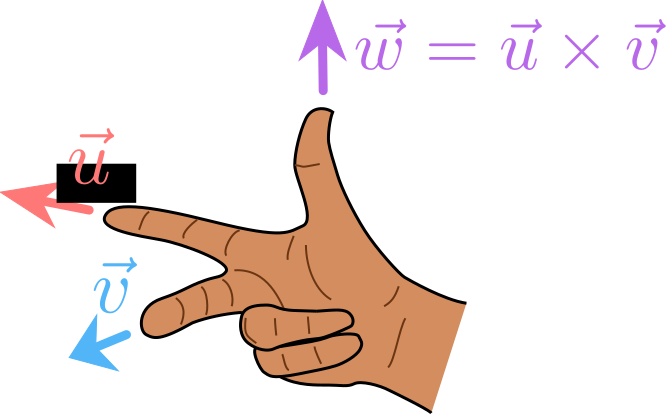
\includegraphics[scale=0.5]{cross_product/rhr.pdf}
\end{figure}

The cross product is \emph{anti-commutative}\index{Anti-commutative}, i.e. changing the order of the vectors results in inverting the product:
\begin{equation*}
  \pcross{u}{v} = -\pcross{v}{u}
\end{equation*}

When the vectors are given as column vectors $\vec{u}=\colvec{3}{u_{x}}{u_{y}}{u_{z}}, \vec{v}=\colvec{3}{v_{x}}{v_{y}}{v_{z}}$, the resulting cross product is
\begin{equation*}
  \pcross{v}{w} = \begin{pmatrix}u_{y}v_{z}-u_{z}v_{y}\\u_{z}v_{x}-u_{x}v_{z}\\u_{x}v_{y}-u_{y}v_{x}\end{pmatrix}
\end{equation*}
\textbf{Write ways of memorizing the cross product}

\begin{example}
  What is the cross product of $\eb{1}=\colvec{3}{1}{0}{0}$ and $\eb{2}=\colvec{3}{0}{1}{0}$?
  \begin{align*}
  \eb{1}\times\eb{2} &= \begin{pmatrix}\cancel{0\cdot0}-\cancel{0\cdot1}\\\cancel{0\cdot0}-\cancel{1\cdot0}\\1\cdot1-\cancel{0\cdot0}\end{pmatrix}\\
  &= \colvec{3}{0}{0}{1}\\
  &= \eb{3}.
  \end{align*}

  Similarly, $\eb{2}\times\eb{3}=\eb{1}$ and $\eb{3}\times\eb{1}=\eb{2}$.
\end{example}

\begin{challange}
  Using component calculation and utilizing the dot product, show that $\pcross{u}{v}$ is indeed orthogonal to both $\vec{u}$ and $\vec{v}$.
\end{challange}
